\documentclass{article}

\usepackage{amsmath}
\usepackage{amsthm}
\usepackage{amssymb}
\usepackage{bm}
\usepackage{bbm}
\usepackage{fancyhdr}
% \usepackage{listings}
\usepackage{cite}
\usepackage{graphicx}
\usepackage{enumitem}
\usepackage{courier}
\usepackage[pdftex,colorlinks=true, urlcolor = blue]{hyperref}
\usepackage{pdfpages}

% Preamble for tikz generated via mathcha.io
\usepackage{physics}
\usepackage{amsmath}
\usepackage{tikz}
\usepackage{mathdots}
\usepackage{yhmath}
\usepackage{cancel}
\usepackage{color}
\usepackage{siunitx}
\usepackage{array}
\usepackage{multirow}
\usepackage{amssymb}
\usepackage{gensymb}
\usepackage{tabularx}
\usepackage{booktabs}
\usetikzlibrary{fadings}
\usetikzlibrary{patterns}
\usetikzlibrary{shadows.blur}
\usetikzlibrary{shapes}


\oddsidemargin 0in \evensidemargin 0in
\topmargin -0.5in \headheight 0.25in \headsep 0.25in
\textwidth 6.5in \textheight 9in
\parskip 6pt \parindent 0in \footskip 20pt

% set the header up
\fancyhead{}
\fancyhead[L]{Stanford Aeronautics \& Astronautics}
\fancyhead[R]{Fall 2020}

%%%%%%%%%%%%%%%%%%%%%%%%%%
\renewcommand\headrulewidth{0.4pt}
\setlength\headheight{15pt}

\usepackage{xparse}
\NewDocumentCommand{\codeword}{v}{%
\texttt{\textcolor{blue}{#1}}%
}

\usepackage{xcolor}
\setlength{\parindent}{0in}

\title{AA 274A: Principles of Robot Autonomy I \\ Problem Set 4 Model}
\author{Name: Li Quan Khoo     \\ SUID: lqkhoo (06154100)}
\date{\today}

\begin{document}

\maketitle
\pagestyle{fancy} 

\section*{Problem 1: EKF Localization}
\begin{enumerate}[label=(\roman*)]
\item % (i)
(code). This written part is not required by the question, but I'll setup the problem here anyway since this is way too much for comments in code, and the derivation is neither in the notes or slides.

\textbf{Given:} A unicycle model with generalized coordinates and instantaneous control vector:
\begin{equation}
\mathbf{x}(t)=
\begin{bmatrix}
x(t) \\ y(t) \\ \theta(t)
\end{bmatrix}
\quad , \quad
\mathbf{u}(t) =
\begin{bmatrix}
V(t) \\ \omega(t)
\end{bmatrix}
\end{equation}

\textbf{Given:} Continuous unicycle model dynamics:
\begin{equation}
\begin{aligned}
\dot{x}(t) &= V(t) \cos(\theta(t)) \\
\dot{y}(t) &= V(t) \sin(\theta(t)) \\
\dot{\theta}(t) &= \omega(t)
\end{aligned}
\end{equation}

For clarity, we denote the value of a variable at discrete time step using subscript $t$ from now on.

\textbf{To find:} Discrete-time state transition model

\begin{equation}
\mathbf{x}_t = g(\mathbf{x}_{t-1}, \mathbf{u}_t)
\end{equation}

$g$ can be interpreted as our belief of the state variables after taking control $\mathbf{u}$ from state $\mathbf{x}_{t-1}$. $\mathbf{x}_t$ is not directly observable due to uncertainty, but assuming $g$ is well-behaved i.e. continuous etc., for small time steps $\Delta t$, we may rely on local similarity in order to approximate it. Let $\tilde{\mathbf{x}}_{t-1}$ and $\tilde{\mathbf{u}}_t$ be small perturbations about $\mathbf{x}_{t-1}$ and $\mathbf{u}_t$. We can use the (multivariate) Taylor series approximation up to first order terms:

\begin{equation}
\begin{aligned}
\mathbf{x}_t = g(\mathbf{x}_{t-1}, \mathbf{u}_t) \approx \tilde{\mathbf{x}}_t &= g(\tilde{\mathbf{x}}_{t-1}, \tilde{\mathbf{u}}_t) \\
&\approx g(\mathbf{x}_{t-1}, \mathbf{u}_t)
+ G_{x,t}(\mathbf{x}_{t-1}, \mathbf{u}_t)\cdot (\tilde{\mathbf{x}}_{t-1} - \mathbf{x}_{t-1})
+ G_{u,t}(\mathbf{x}_{t-1}, \mathbf{u}_t)\cdot (\tilde{\mathbf{u}}_t - \mathbf{u}_t)
\end{aligned}
\end{equation}

where $G_x$ and $G_u$ are Jacobians.

We also assume a zero-order hold on $\mathbf u$, i.e. $\mathbf{u}$ is constant over some time period $\Delta t$. For small $\Delta t$ this is a good approximation. In order to approximate $\mathbf{x}_t$, we find $\tilde{\mathbf{x}}_t$ by discretizing the continuous model using small $\Delta t$ and by using the zero-order hold.

\begin{equation}
\begin{aligned}
\mathbf{x_t} \approx \tilde{\mathbf{x}}_t &= \mathbf{x}_{t-1} + \Delta \mathbf{x} \\
&= \mathbf{x}_{t-1} + \int_0^{\Delta t} \mathbf{\dot x}_{t-1} d\tau
\end{aligned}
\end{equation}

Individually then,
\begin{equation}
\begin{aligned}
\tilde \theta_t &= \theta_{t-1} + \int_0^{\Delta t} \omega_t \; d\tau \;,\quad \omega_t \; \text{constant} \\
&= \theta_{t-1} + \omega_t \tau \big\rvert_0^{\Delta t} \\
&= \theta_{t-1} + \omega_t \Delta t
\end{aligned}
\end{equation}

Because $\theta$ is varying with time, we can follow the hint (on Piazza) and make the substitution $dt = \frac{1}{\omega_t} d\theta$. And thus $\Delta \theta = \omega_t \Delta t$.
\begin{equation}
\begin{aligned}
\tilde x_t &= x_{t-1} + \int_0^{\Delta t} \dot{x}_{t-1} \; d\tau \\
&= x_{t-1} + \int_{\tau=0}^{\tau=\Delta t} V_t \cos(\theta_\tau) \; d\tau \;,\quad V_t \; \text{constant} \\
&= x_{t-1} + \int_{\theta=\theta_{t-1}}^{\theta=\theta_{t-1}+\Delta \theta} V_t\cos(\theta) \cdot \frac{1}{\omega_t} d\theta \\
&= x_{t-1} + \frac{V_t}{\omega_t}\sin(\theta) \Big\rvert_{\theta=\theta_{t-1}}^{\theta=\theta_{t-1}+\Delta \theta} \\
&= x_{t-1} + \frac{V_t}{\omega_t} \Big[ \sin(\theta_{t-1} + \omega_t\Delta t) - \sin(\theta_{t-1}) \Big]
\end{aligned}
\end{equation}

Alternatively, we arrive at the same result by integrating directly wrt $d\tau$ by explicitly considering the passage of time inside the cosine term. As $\tau$ varies, $\theta_\tau$ varies proportionally ($\because\omega_t$ constant) starting from $\theta_{t-1}$ when $\tau=0$ at the rate of $\omega_t \tau$. Therefore:
\begin{equation}
\begin{aligned}
\tilde x_t &= x_{t-1} + \int_0^{\Delta t} \dot{x}_{t-1} \; d\tau \\
&= x_{t-1} + \int_0^{\Delta t} V_t \cos(\theta_\tau) \; d\tau \;,\quad V_t \; \text{constant} \\
&= x_{t-1} + V_t \int_0^{\Delta t} \cos(\theta_{t-1} + \omega_t\tau) \; d\tau \\
&= x_{t-1} + \frac{V_t}{\omega_t} \int_0^{\Delta t} \omega_t \cdot \cos(\theta_{t-1} + \omega_t\tau) \; d\tau \\
&= x_{t-1} + \frac{V_t}{\omega_t} \sin(\theta_{t-1} + \omega_t\tau) \Big\rvert_0^{\Delta t} \\
&= x_{t-1} + \frac{V_t}{\omega_t} \Big[ \sin(\theta_{t-1} + \omega_t\Delta t) - \sin(\theta_{t-1}) \Big]
\end{aligned}
\end{equation}

Likewise,
\begin{equation}
\begin{aligned}
\tilde y_t &= y_{t-1} + \int_0^{\Delta t} \dot{y}_{t-1} \; d\tau \\
&= y_{t-1} + \int_0^{\Delta t} V_t \sin(\theta_\tau) \; d\tau \\
&= y_{t-1} + \frac{V_t}{\omega_t} \int_0^{\Delta t} \omega_t \cdot \sin(\theta_{t-1} + \omega_t\tau) \; d\tau \\
&= y_{t-1} - \frac{V_t}{\omega_t} \Big[ \cos(\theta_{t-1} + \omega_t\Delta t) - \cos(\theta_{t-1}) \Big]
\end{aligned}
\end{equation}

The Jacobian $G_x$ at time $t$ is then
\begin{equation}
G_{x,t}
= \frac{\partial \mathbf{x}_t}{\partial \mathbf{x}_t}
\approx \frac{\partial \tilde{\mathbf{x}}_t}{\partial \tilde{\mathbf{x}}_t}
= \begin{bmatrix}
1 & 0 & \dfrac{\partial \tilde x}{\partial \tilde \theta} \\[6pt]
0 & 1 & \dfrac{\partial \tilde y}{\partial \tilde \theta} \\[6pt]
0 & 0 & 1
\end{bmatrix}_t
\end{equation}

where

\begin{equation}
\begin{aligned}
\frac{\partial \tilde x_t}{\partial \tilde \theta_t}
&= \frac{\partial}{\partial \tilde \theta_t} \Bigg( x_{t-1} + \frac{V_t}{\omega_t} \Big[ \sin(\theta_{t-1} + \omega_t\Delta t) - \sin(\theta_{t-1}) \Big] \Bigg) \\
&= \frac{V_t}{\omega_t} \Big[ \cos(\theta_{t-1} + \omega_t \Delta t) - \cos(\theta_{t-1}) \Big] \\
\frac{\partial \tilde y_t}{\partial \tilde \theta_t}
&= \frac{\partial}{\partial \tilde \theta_t} \Bigg( y_{t-1} - \frac{V_t}{\omega_t} \Big[ \cos(\theta_{t-1} + \omega_t\Delta t) - \cos(\theta_{t-1}) \Big] \Bigg) \\
&= \frac{V_t}{\omega_t} \Big[ \sin(\theta_{t-1} + \omega_t \Delta t) - \sin(\theta_{t-1}) \Big]
\end{aligned}
\end{equation}

Likewise, the Jacobian $G_u$ at time $t$ is
\begin{equation}
G_{u,t}
= \frac{\partial \mathbf{x}_t}{\partial \mathbf{u}_t}
\approx \frac{\partial \tilde{\mathbf{x}}_t}{\partial \tilde{\mathbf{u}}_t}
= \begin{bmatrix}
\dfrac{\partial \tilde x}{\partial \tilde V} & \dfrac{\partial \tilde x}{\partial \tilde \omega} \\[6pt]
\dfrac{\partial \tilde y}{\partial \tilde V} & \dfrac{\partial \tilde y}{\partial \tilde \omega} \\[6pt]
\dfrac{\partial \tilde \theta}{\partial \tilde V} & \dfrac{\partial \tilde \theta}{\partial \tilde \omega} \\
\end{bmatrix}_t
\end{equation}

where

\begin{equation}
\begin{aligned}
\frac{\partial \tilde x_t}{\partial \tilde V_t}
&= \frac{\partial}{\partial \tilde V_t} \Bigg( x_{t-1} + \frac{V_t}{\omega_t} \Big[ \sin(\theta_{t-1} + \omega_t\Delta t) - \sin(\theta_{t-1}) \Big] \Bigg) \\
&= \frac{1}{\omega_t} \Big[ \sin(\theta_{t-1} + \omega_t\Delta t) - \sin(\theta_{t-1}) \Big]
\\
\frac{\partial \tilde y_t}{\partial \tilde V_t}
&= -\frac{1}{\omega_t} \Big[ \cos(\theta_{t-1} + \omega_t\Delta t) - \cos(\theta_{t-1}) \Big]
\\
\frac{\partial \tilde \theta_t}{\partial \tilde V_t} &= 0 \\
\frac{\partial \tilde x_t}{\partial \tilde \omega_t}
&= \frac{\partial}{\partial \tilde \omega_t} \Bigg( x_{t-1} + \frac{V_t}{\omega_t} \Big[ \sin(\theta_{t-1} + \omega_t\Delta t) - \sin(\theta_{t-1}) \Big] \Bigg) \\
&= \frac{\partial}{\partial \tilde \omega_t} \Bigg( \frac{V_t}{\omega_t}\sin(\theta_{t-1} + \omega_t\Delta t) - \frac{V_t}{\omega_t}\sin(\theta_{t-1}) \Bigg) \\
&= -\frac{V_t}{\omega_t^2} \sin(\theta_{t-1} + \omega_t\Delta t) + \frac{V_t}{\omega_t}\cos(\theta_{t-1} + \omega_t\Delta t) \cdot \Delta t + \frac{V_t}{\omega_t^2}\sin(\theta_{t-1}) \\
&= \frac{V_t}{\omega_t^2} \Big [ \sin(\theta_{t-1}) - \sin(\theta_{t-1} + \omega_t\Delta t) + \omega_t \Delta t \cos(\theta_{t-1} + \omega_t\Delta t) \Big]
\\
\frac{\partial \tilde y_t}{\partial \tilde \omega_t}
&= \frac{\partial}{\partial \tilde \omega_t} \Bigg( -\frac{V_t}{\omega_t}\cos(\theta_{t-1} + \omega_t\Delta t) + \frac{V_t}{\omega_t}\cos(\theta_{t-1}) \Bigg) \\
&= \frac{V_t}{\omega_t^2}\cos(\theta_{t-1} + \omega_t\Delta t) + \frac{V_t}{\omega_t}\sin(\theta_{t-1} + \omega_t\Delta t) \cdot \Delta t - \frac{V_t}{\omega_t^2}\cos(\theta_{t-1}) \\
&= \frac{V_t}{\omega_t^2} \Big [ \cos(\theta_{t-1} + \omega_t\Delta t) - \cos(\theta_{t-1}) + \omega_t \Delta t \sin(\theta_{t-1} + \omega_t\Delta t) \Big]
\\
\frac{\partial \tilde \theta_t}{\partial \tilde \omega_t}
&= \frac{\partial}{\partial \tilde \omega_t} \Bigg( \theta_{t-1} + \omega_t \Delta t \Bigg) = \Delta t
\end{aligned}
\end{equation}

As hinted in the question, $\tilde x_t$, $\tilde y_t$, as well as their partial derivatives have $\omega_t$ in the denominator and are thus indeterminate in their current form as $\omega_t \to 0$. However, these terms are composed from continuous functions; by inspection, $V_t$ and $\omega_t$ are our continuous control variables, $\sin$ and $\cos$ are continuous. Therefore we may apply l'Hopital's rule to evaluate them at the limit where $\omega_t = 0$.

\pagebreak

\begin{equation}
\begin{aligned}
\lim_{\omega_t \to 0} x_t
&= x_{t-1} + \lim_{\omega_t \to 0} \frac{V_t \big(\sin(\theta_{t-1} + \omega_t\Delta t) - \sin(\theta_{t-1})\big)}{\omega_t} \\
&= x_{t-1} + \lim_{\omega_t \to 0} \frac{ \frac{\partial}{\partial \omega_t} V_t \big(\sin(\theta_{t-1} + \omega_t\Delta t) - \sin(\theta_{t-1})\big)}{ \frac{\partial}{\partial \omega_t} \omega_t} \quad, \quad \text{l'Hopital's rule} \\
&= x_{t-1} + \lim_{\omega_t \to 0} \frac{V_t \Delta t \cos(\theta_{t-1} + \omega_t \Delta t)}{1} \\
&= x_{t-1} + V_t \Delta t \cos(\theta_{t-1} + \omega_t \Delta t) \Big\rvert_{\omega_t = 0} \\
&= x_{t-1} + V_t \Delta t \cos(\theta_{t-1})
\\
\lim_{\omega_t \to 0} y_t
&= y_{t-1} + \lim_{\omega_t \to 0} - \frac{V_t}{\omega_t} \Big[ \cos(\theta_{t-1} + \omega_t\Delta t) - \cos(\theta_{t-1}) \Big] \\
&= y_{t-1} + V_t \Delta t \sin(\theta_{t-1})
\\
\lim_{\omega_t \to 0} \frac{\partial \tilde x_t}{\partial \tilde \theta_t}
&= \lim_{\omega_t \to 0} \frac{V_t}{\omega_t} \Big[ \cos(\theta_{t-1} + \omega_t \Delta t) - \cos(\theta_{t-1}) \Big] \\
&= -V_t \Delta t \sin(\theta_{t-1})
\\
\lim_{\omega_t \to 0} \frac{\partial \tilde y_t}{\partial \tilde \theta_t}
&= \lim_{\omega_t \to 0} \frac{V_t}{\omega_t} \Big[ \sin(\theta_{t-1} + \omega_t \Delta t) - \sin(\theta_{t-1}) \Big] \\
&= V_t \Delta t \cos(\theta_{t-1})
\\
\lim_{\omega_t \to 0} \frac{\partial \tilde x_t}{\partial \tilde V_t}
&= \lim_{\omega_t \to 0} \frac{1}{\omega_t} \Big[ \sin(\theta_{t-1} + \omega_t\Delta t) - \sin(\theta_{t-1}) \Big] \\
&= \Delta t \cos(\theta_{t-1})
\\
\lim_{\omega_t \to 0} \frac{\partial \tilde y_t}{\partial \tilde V_t}
&= \lim_{\omega_t \to 0} -\frac{1}{\omega_t} \Big[ \cos(\theta_{t-1} + \omega_t\Delta t) - \cos(\theta_{t-1}) \Big] \\
&= \Delta t \sin(\theta_{t-1})
\\
\lim_{\omega_t \to 0} \frac{\partial \tilde x_t}{\partial \tilde \omega_t}
&= \lim_{\omega_t \to 0} \frac{V_t}{\omega_t^2} \Big [ \sin(\theta_{t-1}) - \sin(\theta_{t-1} + \omega_t\Delta t) + \omega_t \Delta t \cos(\theta_{t-1} + \omega_t\Delta t) \Big] \\
&= \lim_{\omega_t \to 0} \frac{V_t}{2 \omega_t} \Big[ \underbrace{- \Delta t\cos(\theta_{t-1} + \omega_t \Delta t) + \Delta t\cos(\theta_{t-1} + \omega_t \Delta t)}_{=0} - \omega_t (\Delta t)^2 \sin(\theta_{t-1} + \omega_t \Delta t) \Big] \\
&= \frac{V_t}{2} \Big[ -(\Delta t)^2 \sin(\theta_{t-1} + \omega_t \Delta t) - \omega_t (\Delta t)^3\cos(\theta_{t-1} + \omega_t \Delta t) \Big] \Big\rvert_{\omega_t = 0}\\
&= -\frac{V_t (\Delta t)^2}{2} \sin(\theta_{t-1})
\\
\lim_{\omega_t \to 0} \frac{\partial \tilde y_t}{\partial \tilde \omega_t} 
&= \lim_{\omega_t \to 0} \frac{V_t}{\omega_t^2} \Big [ \cos(\theta_{t-1} + \omega_t\Delta t) - \cos(\theta_{t-1}) + \omega_t \Delta t \sin(\theta_{t-1} + \omega_t\Delta t) \Big] \\
&= \lim_{\omega_t \to 0} \frac{V_t}{2 \omega_t} \Big[ \underbrace{-\Delta t \sin(\theta_{t-1} + \omega_t \Delta t) + \Delta t \sin(\theta_{t-1} + \omega_t \Delta t)}_{=0} + \omega_t(\Delta t)^2 \cos(\theta_{t-1} + \omega_t \Delta t) \Big] \\
&= \frac{V_t}{2} \Big[ (\Delta t)^2\cos(\theta_{t-1} + \omega_t \Delta t) - \omega_t (\Delta t)^3 \sin(\theta_{t-1} + \omega_t \Delta t) \Big] \Big\rvert_{\omega_t=0} \\
&= \frac{V_t (\Delta t)^2}{2} \cos(\theta_{t-1})
\end{aligned}
\end{equation}

\pagebreak

\item % (ii)
(code) Following the pset, since the EKF assumes Gaussian belief, our unobservable state $\mathbf{x}_t$ can be assumed to be distributed as $\mathbf{x}_t \sim \mathcal{N}(\mathbf{x}_{t-1}, \Sigma_{t-1})$. Modeling the noise resulting from approximating the dynamics as $\upsilon \sim \mathcal{N}(0, R)$, our best prediction $\bar{\mathbf{x}}_t$ i.e. the mean of $\mathbf{x}_t$ is thus represented in the following EKF assignment step:

\begin{equation}
\begin{aligned}
\bar{\mathbf{x}}_t = g(\mathbf{x}_{t-1}, \mathbf{u}_t) &\leftarrow \tilde{\mathbf{x}} = g(\tilde{\mathbf{x}}_{t-1}, \tilde{\mathbf{u}}_t) \\
\bar{\Sigma}_t &\leftarrow G_{x,t} \Sigma_{t-1} G_{x,t}^\mathsf{T} + \Delta t \cdot G_{u,t} R G_{u,t}^\mathsf{T}
\end{aligned}
\end{equation}

\item % (iii)
(code) Our task is to recover ${}^C\alpha$ and ${}^C r$, i.e. the parameters of the line of interest expressed in Camera coordinates. First consider the diagram below.

Red and green axes represent coordinate frames of the World, Robot, and Camera. We can see that ${}^C\alpha$ is the angle $\alpha$ after subtracting from the relative frame rotations going from the World to Robot to Camera frame, i.e.

\begin{equation}
{}^C\alpha = \alpha - ({}^W\theta_{robot} + {}^R\theta_{cam})
\end{equation}

\tikzset{every picture/.style={line width=0.75pt}} %set default line width to 0.75pt        

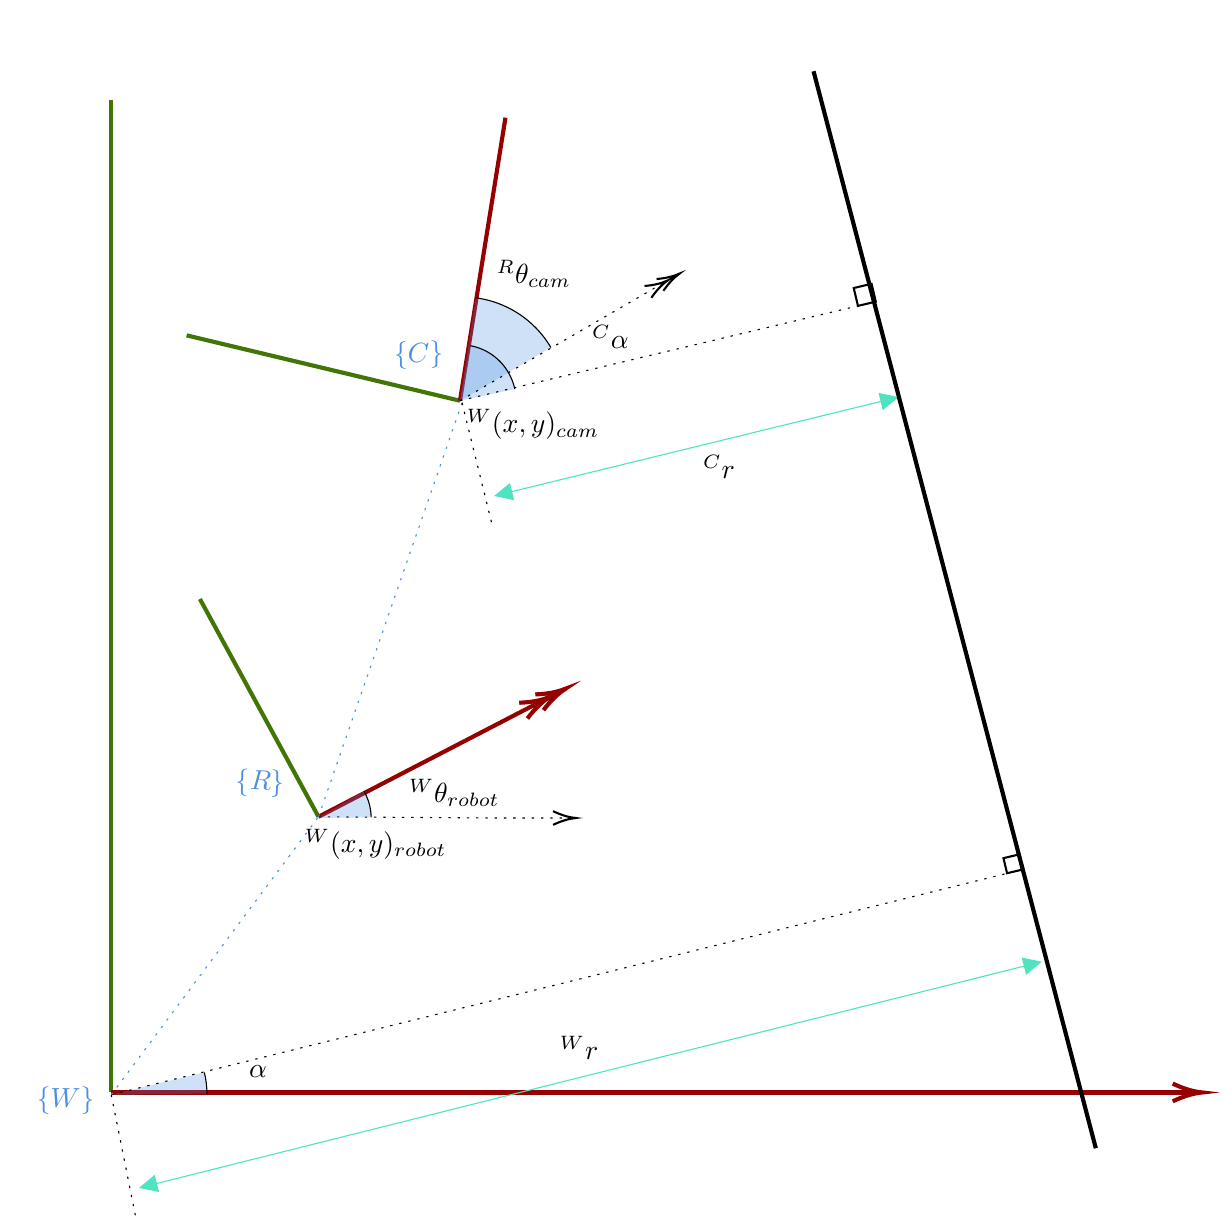
\begin{tikzpicture}[x=0.75pt,y=0.75pt,yscale=-1,xscale=1]
%uncomment if require: \path (0,591); %set diagram left start at 0, and has height of 591

%Straight Lines [id:da3125945440474338] 
\draw [color={rgb, 255:red, 65; green, 117; blue, 5 }  ,draw opacity=1 ][fill={rgb, 255:red, 74; green, 144; blue, 226 }  ,fill opacity=1 ][line width=1.5]    (84.65,24.41) -- (84.65,502.51) ;
%Straight Lines [id:da2966783903800445] 
\draw [color={rgb, 255:red, 150; green, 0; blue, 0 }  ,draw opacity=1 ][fill={rgb, 255:red, 74; green, 144; blue, 226 }  ,fill opacity=1 ][line width=1.5]    (607.27,502.51) -- (84.65,502.51) ;
\draw [shift={(610.27,502.51)}, rotate = 180] [color={rgb, 255:red, 150; green, 0; blue, 0 }  ,draw opacity=1 ][line width=1.5]    (14.21,-4.28) .. controls (9.04,-1.82) and (4.3,-0.39) .. (0,0) .. controls (4.3,0.39) and (9.04,1.82) .. (14.21,4.28)   ;
%Shape: Arc [id:dp4520577678034412] 
\draw  [draw opacity=0][fill={rgb, 255:red, 74; green, 144; blue, 226 }  ,fill opacity=0.27 ] (129.49,492.84) .. controls (130.28,496.12) and (130.72,499.53) .. (130.76,503.04) -- (84.65,503.64) -- cycle ; \draw   (129.49,492.84) .. controls (130.28,496.12) and (130.72,499.53) .. (130.76,503.04) ;
%Straight Lines [id:da49309395450716864] 
\draw  [dash pattern={on 0.84pt off 2.51pt}]  (84.65,503.64) -- (523.49,395.16) ;
%Shape: Rectangle [id:dp4229332944930504] 
\draw  [line width=0.75]  (516.23,396.88) -- (514.51,389.62) -- (521.77,387.89) -- (523.49,395.16) -- cycle ;
%Straight Lines [id:da8914089624231336] 
\draw [color={rgb, 255:red, 65; green, 117; blue, 5 }  ,draw opacity=1 ][line width=1.5]    (127.36,264.76) -- (184.5,369.69) ;
%Straight Lines [id:da8374459467756974] 
\draw [color={rgb, 255:red, 150; green, 0; blue, 0 }  ,draw opacity=1 ][line width=1.5]    (303.52,307.99) -- (184.5,369.69) ;
\draw [shift={(303.52,307.99)}, rotate = 152.6] [color={rgb, 255:red, 150; green, 0; blue, 0 }  ,draw opacity=1 ][line width=1.5]    (22.93,-4.28) .. controls (17.76,-1.82) and (13.02,-0.39) .. (8.72,0) .. controls (13.02,0.39) and (17.76,1.82) .. (22.93,4.28)(14.21,-4.28) .. controls (9.04,-1.82) and (4.3,-0.39) .. (0,0) .. controls (4.3,0.39) and (9.04,1.82) .. (14.21,4.28)   ;
%Straight Lines [id:da33282737778346605] 
\draw  [dash pattern={on 0.84pt off 2.51pt}]  (184.5,369.69) -- (270.09,370.28) -- (306.45,370.28) ;
\draw [shift={(308.45,370.28)}, rotate = 180] [color={rgb, 255:red, 0; green, 0; blue, 0 }  ][line width=0.75]    (10.93,-3.29) .. controls (6.95,-1.4) and (3.31,-0.3) .. (0,0) .. controls (3.31,0.3) and (6.95,1.4) .. (10.93,3.29)   ;
%Shape: Arc [id:dp7618276180320753] 
\draw  [draw opacity=0][fill={rgb, 255:red, 74; green, 144; blue, 226 }  ,fill opacity=0.27 ] (206.41,357.42) .. controls (208.55,361.11) and (209.8,365.39) .. (209.85,369.94) -- (184.14,370.28) -- cycle ; \draw   (206.41,357.42) .. controls (208.55,361.11) and (209.8,365.39) .. (209.85,369.94) ;
%Straight Lines [id:da653574132076578] 
\draw [color={rgb, 255:red, 74; green, 144; blue, 226 }  ,draw opacity=1 ] [dash pattern={on 0.84pt off 2.51pt}]  (84.65,503.64) -- (184.5,369.69) ;

%Straight Lines [id:da8566079839197343] 
\draw [color={rgb, 255:red, 74; green, 144; blue, 226 }  ,draw opacity=1 ] [dash pattern={on 0.84pt off 2.51pt}]  (184.5,369.69) -- (253.66,170.23) ;
%Straight Lines [id:da42171131167454723] 
\draw [color={rgb, 255:red, 65; green, 117; blue, 5 }  ,draw opacity=1 ][fill={rgb, 255:red, 74; green, 144; blue, 226 }  ,fill opacity=1 ][line width=1.5]    (120.96,137.74) -- (252.66,169.23) ;
%Straight Lines [id:da9750993592309116] 
\draw [color={rgb, 255:red, 150; green, 0; blue, 0 }  ,draw opacity=1 ][fill={rgb, 255:red, 74; green, 144; blue, 226 }  ,fill opacity=1 ][line width=1.5]    (274.57,32.87) -- (252.66,169.23) ;
%Shape: Arc [id:dp5977706961904254] 
\draw  [draw opacity=0][fill={rgb, 255:red, 74; green, 144; blue, 226 }  ,fill opacity=0.27 ] (260.27,119.63) .. controls (274.95,121.64) and (288.49,130.03) .. (296.43,143.59) -- (252.66,169.23) -- cycle ; \draw   (260.27,119.63) .. controls (274.95,121.64) and (288.49,130.03) .. (296.43,143.59) ;
%Shape: Arc [id:dp05251841891450337] 
\draw  [draw opacity=0][fill={rgb, 255:red, 74; green, 144; blue, 226 }  ,fill opacity=0.27 ] (257.77,142.73) .. controls (265.29,144.18) and (272.15,148.81) .. (276.2,156.02) .. controls (277.57,158.47) and (278.52,161.03) .. (279.07,163.64) -- (252.66,169.23) -- cycle ; \draw   (257.77,142.73) .. controls (265.29,144.18) and (272.15,148.81) .. (276.2,156.02) .. controls (277.57,158.47) and (278.52,161.03) .. (279.07,163.64) ;
%Straight Lines [id:da9547262639369065] 
\draw  [dash pattern={on 0.84pt off 2.51pt}]  (252.66,169.23) -- (358.48,107.96) ;
\draw [shift={(358.48,107.96)}, rotate = 509.93] [color={rgb, 255:red, 0; green, 0; blue, 0 }  ][line width=0.75]    (17.64,-3.29) .. controls (13.66,-1.4) and (10.02,-0.3) .. (6.71,0) .. controls (10.02,0.3) and (13.66,1.4) .. (17.64,3.29)(10.93,-3.29) .. controls (6.95,-1.4) and (3.31,-0.3) .. (0,0) .. controls (3.31,0.3) and (6.95,1.4) .. (10.93,3.29)   ;
%Straight Lines [id:da9209398119053456] 
\draw  [dash pattern={on 0.84pt off 2.51pt}]  (252.66,169.23) -- (453,121.5) ;
%Straight Lines [id:da9311655693647147] 
\draw [color={rgb, 255:red, 0; green, 0; blue, 0 }  ,draw opacity=1 ] [dash pattern={on 0.84pt off 2.51pt}]  (253.66,170.23) -- (268,228.5) ;

%Straight Lines [id:da44006225641206265] 
\draw [color={rgb, 255:red, 80; green, 227; blue, 194 }  ,draw opacity=1 ]   (272,214.41) -- (461.09,168.21) ;
\draw [shift={(464,167.5)}, rotate = 526.27] [fill={rgb, 255:red, 80; green, 227; blue, 194 }  ,fill opacity=1 ][line width=0.08]  [draw opacity=0] (8.93,-4.29) -- (0,0) -- (8.93,4.29) -- cycle    ;
\draw [shift={(269.09,215.12)}, rotate = 346.27] [fill={rgb, 255:red, 80; green, 227; blue, 194 }  ,fill opacity=1 ][line width=0.08]  [draw opacity=0] (8.93,-4.29) -- (0,0) -- (8.93,4.29) -- cycle    ;
%Shape: Rectangle [id:dp28375929983845727] 
\draw  [line width=0.75]  (444.4,123.54) -- (442.36,114.94) -- (450.96,112.9) -- (453,121.5) -- cycle ;
%Straight Lines [id:da9749283234703954] 
\draw [line width=1.5]    (423,10.5) -- (559,529.38) ;
%Straight Lines [id:da13884579717265644] 
\draw [color={rgb, 255:red, 80; green, 227; blue, 194 }  ,draw opacity=1 ]   (100.91,547.77) -- (530.09,440.23) ;
\draw [shift={(533,439.5)}, rotate = 525.9300000000001] [fill={rgb, 255:red, 80; green, 227; blue, 194 }  ,fill opacity=1 ][line width=0.08]  [draw opacity=0] (8.93,-4.29) -- (0,0) -- (8.93,4.29) -- cycle    ;
\draw [shift={(98,548.5)}, rotate = 345.93] [fill={rgb, 255:red, 80; green, 227; blue, 194 }  ,fill opacity=1 ][line width=0.08]  [draw opacity=0] (8.93,-4.29) -- (0,0) -- (8.93,4.29) -- cycle    ;
%Straight Lines [id:da21037991729314842] 
\draw  [dash pattern={on 0.84pt off 2.51pt}]  (84.65,503.64) -- (98,570.5) ;

% Text Node
\draw (76.61,506.51) node   [align=left] {\begin{minipage}[lt]{41.688984005682464pt}\setlength\topsep{0pt}
	\textcolor[rgb]{0.29,0.56,0.89}{$\{W\}$}
	\end{minipage}};
% Text Node
\draw (149.82,488.39) node [anchor=north west][inner sep=0.75pt]   [align=left] {$\alpha$};
% Text Node
\draw (299.5,474) node [anchor=north west][inner sep=0.75pt] [align=left] {${}^W r$};
% Text Node
\draw (368.54,194.31) node [anchor=north west][inner sep=0.75pt]   [align=left] {${}^C r$};
% Text Node
\draw (160.64,353.55) node  [rotate=-1.33,xslant=0] [align=left] {\begin{minipage}[lt]{23.788530321472685pt}\setlength\topsep{0pt}
	{$\textcolor[rgb]{0.29,0.56,0.89}{\{R\}}$}
	\end{minipage}};
% Text Node
\draw (257.2,358.33) node   [align=left] {\begin{minipage}[lt]{43.61420332583847pt}\setlength\topsep{0pt}
	{${}^W\theta_{robot}$}
\end{minipage}};
% Text Node
\draw (176.66,374.23) node [anchor=north west][inner sep=0.75pt] [align=left] {${}^W(x,y)_{robot}$};
% Text Node
\draw (236.84,147.2) node  [rotate=-359.62,xslant=-0.01] [align=left] {\begin{minipage}[lt]{23.99426982578997pt}\setlength\topsep{0pt}
	{$\textcolor[rgb]{0.29,0.56,0.89}{\{C\}}$}
	\end{minipage}};
% Text Node
\draw (292.79,108.07) node   [align=left] {\begin{minipage}[lt]{33.48046385316968pt}\setlength\topsep{0pt}
{${}^R \theta_{cam}$}
\end{minipage}};
% Text Node
\draw (315.07,131.64) node [anchor=north west][inner sep=0.75pt]   [align=left] {${}^C \alpha$};
% Text Node
\draw (254.66,172.23) node [anchor=north west][inner sep=0.75pt]   [align=left] {${}^W( x,y)_{cam}$};

\end{tikzpicture}

\pagebreak

It is more difficult to recover ${}^C r$, as we cannot simply perform a frame translation and rotation because the endpoints on the line of interest are different. We approach this geometrically. Now consider the more detailed diagram below:



\tikzset{every picture/.style={line width=0.75pt}} %set default line width to 0.75pt        

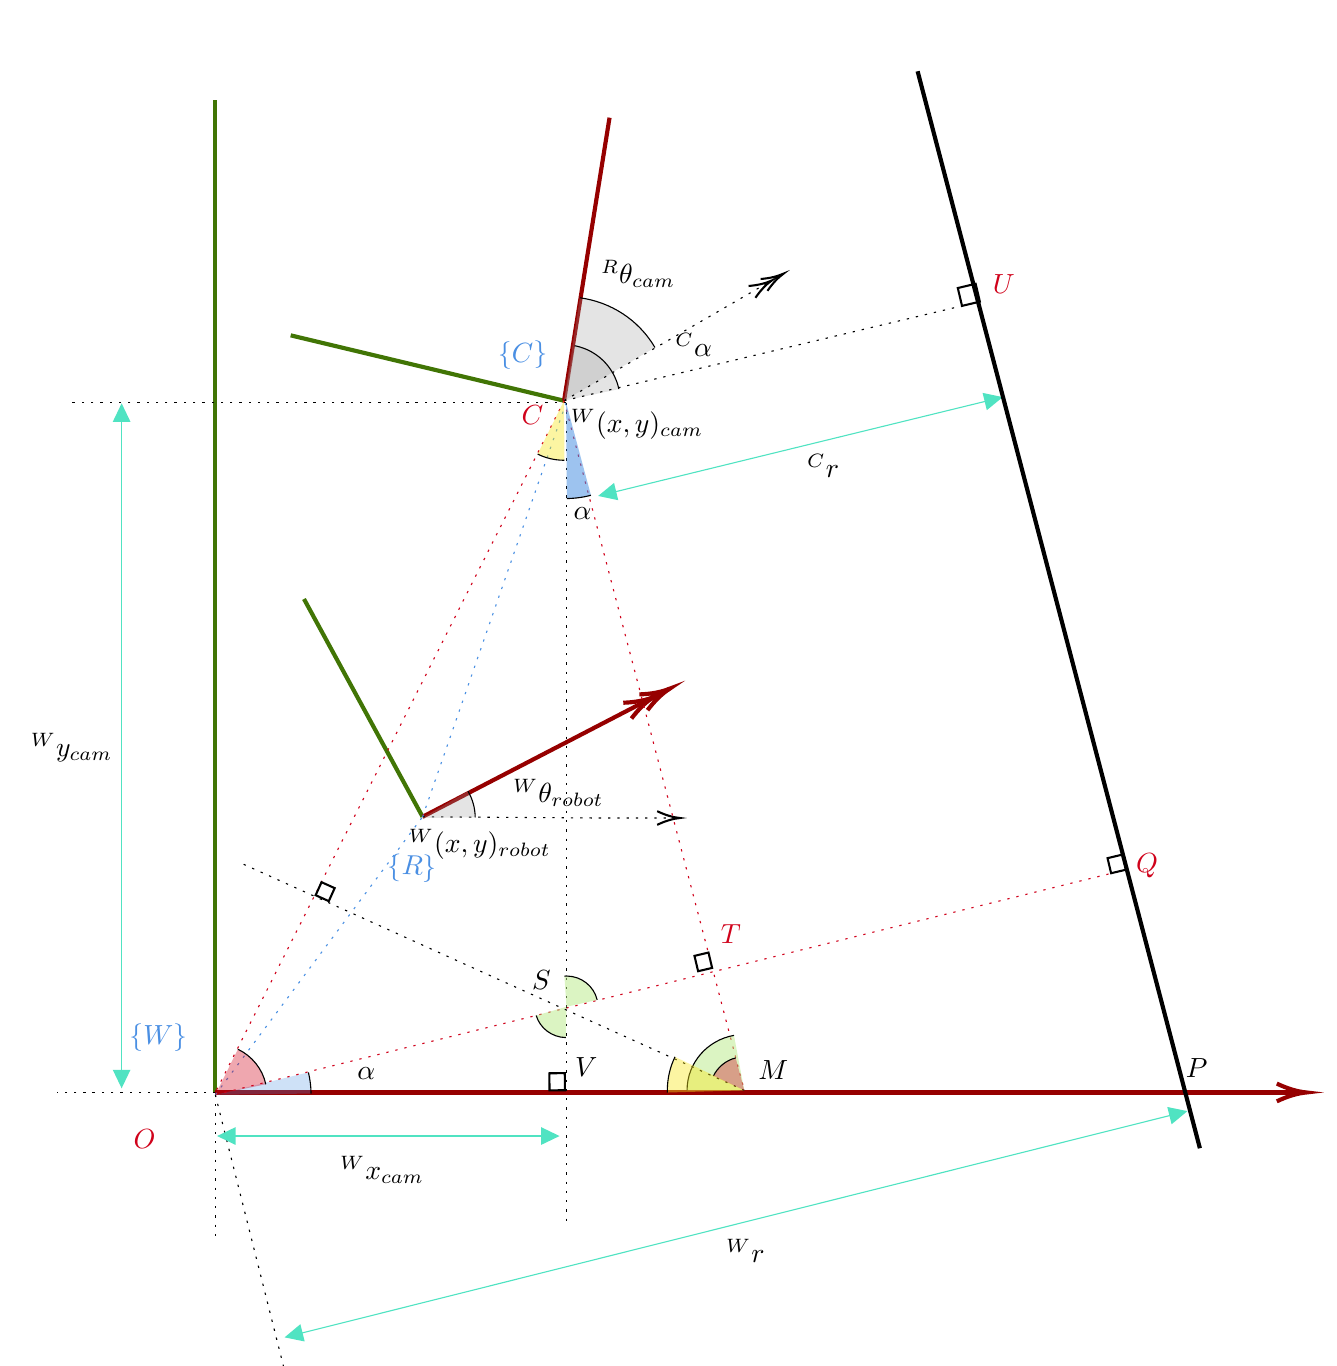
\begin{tikzpicture}[x=0.75pt,y=0.75pt,yscale=-1,xscale=1]
%uncomment if require: \path (0,662); %set diagram left start at 0, and has height of 662

%Straight Lines [id:da3934086400282608] 
\draw [color={rgb, 255:red, 65; green, 117; blue, 5 }  ,draw opacity=1 ][fill={rgb, 255:red, 74; green, 144; blue, 226 }  ,fill opacity=1 ][line width=1.5]    (127.65,29.91) -- (127.65,508.01) ;
%Straight Lines [id:da8050713881919771] 
\draw [color={rgb, 255:red, 150; green, 0; blue, 0 }  ,draw opacity=1 ][fill={rgb, 255:red, 74; green, 144; blue, 226 }  ,fill opacity=1 ][line width=1.5]    (650.27,508.01) -- (127.65,508.01) ;
\draw [shift={(653.27,508.01)}, rotate = 180] [color={rgb, 255:red, 150; green, 0; blue, 0 }  ,draw opacity=1 ][line width=1.5]    (14.21,-4.28) .. controls (9.04,-1.82) and (4.3,-0.39) .. (0,0) .. controls (4.3,0.39) and (9.04,1.82) .. (14.21,4.28)   ;
%Shape: Arc [id:dp7889101967904575] 
\draw  [draw opacity=0][fill={rgb, 255:red, 74; green, 144; blue, 226 }  ,fill opacity=0.27 ] (172.49,498.34) .. controls (173.28,501.62) and (173.72,505.03) .. (173.76,508.54) -- (127.65,509.14) -- cycle ; \draw   (172.49,498.34) .. controls (173.28,501.62) and (173.72,505.03) .. (173.76,508.54) ;
%Straight Lines [id:da8575813604499853] 
\draw [color={rgb, 255:red, 208; green, 2; blue, 27 }  ,draw opacity=1 ] [dash pattern={on 0.84pt off 2.51pt}]  (127.65,509.14) -- (566.49,400.66) ;
%Shape: Rectangle [id:dp5933020737117791] 
\draw  [line width=0.75]  (559.23,402.38) -- (557.51,395.12) -- (564.77,393.39) -- (566.49,400.66) -- cycle ;
%Straight Lines [id:da43498231193660697] 
\draw [color={rgb, 255:red, 65; green, 117; blue, 5 }  ,draw opacity=1 ][line width=1.5]    (170.36,270.26) -- (227.5,375.19) ;
%Straight Lines [id:da19788929521074183] 
\draw [color={rgb, 255:red, 150; green, 0; blue, 0 }  ,draw opacity=1 ][line width=1.5]    (346.52,313.49) -- (227.5,375.19) ;
\draw [shift={(346.52,313.49)}, rotate = 152.6] [color={rgb, 255:red, 150; green, 0; blue, 0 }  ,draw opacity=1 ][line width=1.5]    (22.93,-4.28) .. controls (17.76,-1.82) and (13.02,-0.39) .. (8.72,0) .. controls (13.02,0.39) and (17.76,1.82) .. (22.93,4.28)(14.21,-4.28) .. controls (9.04,-1.82) and (4.3,-0.39) .. (0,0) .. controls (4.3,0.39) and (9.04,1.82) .. (14.21,4.28)   ;
%Straight Lines [id:da12512379790846695] 
\draw  [dash pattern={on 0.84pt off 2.51pt}]  (227.5,375.19) -- (313.09,375.78) -- (349.45,375.78) ;
\draw [shift={(351.45,375.78)}, rotate = 180] [color={rgb, 255:red, 0; green, 0; blue, 0 }  ][line width=0.75]    (10.93,-3.29) .. controls (6.95,-1.4) and (3.31,-0.3) .. (0,0) .. controls (3.31,0.3) and (6.95,1.4) .. (10.93,3.29)   ;
%Shape: Arc [id:dp9198054046584554] 
\draw  [draw opacity=0][fill={rgb, 255:red, 155; green, 155; blue, 155 }  ,fill opacity=0.27 ] (249.41,362.92) .. controls (251.55,366.61) and (252.8,370.89) .. (252.85,375.44) -- (227.14,375.78) -- cycle ; \draw   (249.41,362.92) .. controls (251.55,366.61) and (252.8,370.89) .. (252.85,375.44) ;
%Straight Lines [id:da20735883638067376] 
\draw [color={rgb, 255:red, 74; green, 144; blue, 226 }  ,draw opacity=1 ] [dash pattern={on 0.84pt off 2.51pt}]  (127.65,509.14) -- (227.5,375.19) ;

%Straight Lines [id:da5135388136858381] 
\draw [color={rgb, 255:red, 74; green, 144; blue, 226 }  ,draw opacity=1 ] [dash pattern={on 0.84pt off 2.51pt}]  (227.5,375.19) -- (296.66,175.73) ;
%Straight Lines [id:da23842253594459772] 
\draw [color={rgb, 255:red, 65; green, 117; blue, 5 }  ,draw opacity=1 ][fill={rgb, 255:red, 74; green, 144; blue, 226 }  ,fill opacity=1 ][line width=1.5]    (163.96,143.24) -- (295.66,174.73) ;
%Straight Lines [id:da3846145700813639] 
\draw [color={rgb, 255:red, 150; green, 0; blue, 0 }  ,draw opacity=1 ][fill={rgb, 255:red, 74; green, 144; blue, 226 }  ,fill opacity=1 ][line width=1.5]    (317.57,38.37) -- (295.66,174.73) ;
%Shape: Arc [id:dp7312639822692524] 
\draw  [draw opacity=0][fill={rgb, 255:red, 155; green, 155; blue, 155 }  ,fill opacity=0.27 ] (303.27,125.13) .. controls (317.95,127.14) and (331.49,135.53) .. (339.43,149.09) -- (295.66,174.73) -- cycle ; \draw   (303.27,125.13) .. controls (317.95,127.14) and (331.49,135.53) .. (339.43,149.09) ;
%Shape: Arc [id:dp9667815185322768] 
\draw  [draw opacity=0][fill={rgb, 255:red, 155; green, 155; blue, 155 }  ,fill opacity=0.27 ] (300.77,148.23) .. controls (308.29,149.68) and (315.15,154.31) .. (319.2,161.52) .. controls (320.57,163.97) and (321.52,166.53) .. (322.07,169.14) -- (295.66,174.73) -- cycle ; \draw   (300.77,148.23) .. controls (308.29,149.68) and (315.15,154.31) .. (319.2,161.52) .. controls (320.57,163.97) and (321.52,166.53) .. (322.07,169.14) ;
%Straight Lines [id:da4332012099557956] 
\draw  [dash pattern={on 0.84pt off 2.51pt}]  (295.66,174.73) -- (401.48,113.46) ;
\draw [shift={(401.48,113.46)}, rotate = 509.93] [color={rgb, 255:red, 0; green, 0; blue, 0 }  ][line width=0.75]    (17.64,-3.29) .. controls (13.66,-1.4) and (10.02,-0.3) .. (6.71,0) .. controls (10.02,0.3) and (13.66,1.4) .. (17.64,3.29)(10.93,-3.29) .. controls (6.95,-1.4) and (3.31,-0.3) .. (0,0) .. controls (3.31,0.3) and (6.95,1.4) .. (10.93,3.29)   ;
%Straight Lines [id:da9521767396239376] 
\draw  [dash pattern={on 0.84pt off 2.51pt}]  (295.66,174.73) -- (496,127) ;

%Straight Lines [id:da14161854021053033] 
\draw [color={rgb, 255:red, 208; green, 2; blue, 27 }  ,draw opacity=1 ] [dash pattern={on 0.84pt off 2.51pt}]  (295.66,174.73) -- (382.5,507) ;
%Straight Lines [id:da7316941275917717] 
\draw [color={rgb, 255:red, 80; green, 227; blue, 194 }  ,draw opacity=1 ]   (315,219.91) -- (504.09,173.71) ;
\draw [shift={(507,173)}, rotate = 526.27] [fill={rgb, 255:red, 80; green, 227; blue, 194 }  ,fill opacity=1 ][line width=0.08]  [draw opacity=0] (8.93,-4.29) -- (0,0) -- (8.93,4.29) -- cycle    ;
\draw [shift={(312.09,220.62)}, rotate = 346.27] [fill={rgb, 255:red, 80; green, 227; blue, 194 }  ,fill opacity=1 ][line width=0.08]  [draw opacity=0] (8.93,-4.29) -- (0,0) -- (8.93,4.29) -- cycle    ;
%Shape: Rectangle [id:dp10692268810512973] 
\draw  [line width=0.75]  (487.4,129.04) -- (485.36,120.44) -- (493.96,118.4) -- (496,127) -- cycle ;
%Straight Lines [id:da29757284193133215] 
\draw [line width=1.5]    (466,16) -- (602,534.88) ;
%Straight Lines [id:da3304295558006165] 
\draw [color={rgb, 255:red, 80; green, 227; blue, 194 }  ,draw opacity=1 ]   (163.91,625.27) -- (593.09,517.73) ;
\draw [shift={(596,517)}, rotate = 525.9300000000001] [fill={rgb, 255:red, 80; green, 227; blue, 194 }  ,fill opacity=1 ][line width=0.08]  [draw opacity=0] (8.93,-4.29) -- (0,0) -- (8.93,4.29) -- cycle    ;
\draw [shift={(161,626)}, rotate = 345.93] [fill={rgb, 255:red, 80; green, 227; blue, 194 }  ,fill opacity=1 ][line width=0.08]  [draw opacity=0] (8.93,-4.29) -- (0,0) -- (8.93,4.29) -- cycle    ;
%Straight Lines [id:da30293313656825105] 
\draw  [dash pattern={on 0.84pt off 2.51pt}]  (127.65,509.14) -- (162,646) ;
%Straight Lines [id:da19911994593624893] 
\draw [color={rgb, 255:red, 0; green, 0; blue, 0 }  ,draw opacity=1 ] [dash pattern={on 0.84pt off 2.51pt}]  (296.66,175.73) -- (296.66,571) ;
%Shape: Arc [id:dp4778842949929132] 
\draw  [draw opacity=0][fill={rgb, 255:red, 74; green, 144; blue, 226 }  ,fill opacity=0.54 ] (308.61,220.28) .. controls (304.9,221.27) and (301.01,221.82) .. (297,221.85) -- (296.66,175.73) -- cycle ; \draw   (308.61,220.28) .. controls (304.9,221.27) and (301.01,221.82) .. (297,221.85) ;
%Shape: Rectangle [id:dp2586064388070355] 
\draw  [line width=0.75]  (288.58,498.77) -- (296,498.7) -- (296.08,506.93) -- (288.66,507) -- cycle ;
%Straight Lines [id:da8225660226036944] 
\draw  [dash pattern={on 0.84pt off 2.51pt}]  (127.65,509.14) -- (127.65,578) ;
%Shape: Rectangle [id:dp8912343443918627] 
\draw  [line width=0.75]  (360.25,449.6) -- (358.49,442.2) -- (365.25,440.6) -- (367,448) -- cycle ;
%Straight Lines [id:da5371571449723658] 
\draw [color={rgb, 255:red, 208; green, 2; blue, 27 }  ,draw opacity=1 ] [dash pattern={on 0.84pt off 2.51pt}]  (295.66,174.73) -- (127.65,508.01) ;
%Shape: Arc [id:dp5049176757454987] 
\draw  [draw opacity=0][fill={rgb, 255:red, 208; green, 2; blue, 27 }  ,fill opacity=0.35 ] (138.53,487.19) .. controls (145.31,490.44) and (150.36,496.63) .. (151.96,504.05) -- (127.65,509.14) -- cycle ; \draw   (138.53,487.19) .. controls (145.31,490.44) and (150.36,496.63) .. (151.96,504.05) ;
%Straight Lines [id:da7420408442162774] 
\draw  [dash pattern={on 0.84pt off 2.51pt}]  (127.65,508.01) -- (51.5,508.01) ;
%Straight Lines [id:da04663080177486245] 
\draw  [dash pattern={on 0.84pt off 2.51pt}]  (296.66,175.73) -- (58.5,175.73) ;
%Straight Lines [id:da103218103320035] 
\draw [color={rgb, 255:red, 80; green, 227; blue, 194 }  ,draw opacity=1 ]   (131.5,529) -- (290.5,529) ;
\draw [shift={(293.5,529)}, rotate = 180] [fill={rgb, 255:red, 80; green, 227; blue, 194 }  ,fill opacity=1 ][line width=0.08]  [draw opacity=0] (8.93,-4.29) -- (0,0) -- (8.93,4.29) -- cycle    ;
\draw [shift={(128.5,529)}, rotate = 0] [fill={rgb, 255:red, 80; green, 227; blue, 194 }  ,fill opacity=1 ][line width=0.08]  [draw opacity=0] (8.93,-4.29) -- (0,0) -- (8.93,4.29) -- cycle    ;
%Straight Lines [id:da23956290671679126] 
\draw [color={rgb, 255:red, 80; green, 227; blue, 194 }  ,draw opacity=1 ]   (82.5,503) -- (82.5,179) ;
\draw [shift={(82.5,176)}, rotate = 450] [fill={rgb, 255:red, 80; green, 227; blue, 194 }  ,fill opacity=1 ][line width=0.08]  [draw opacity=0] (8.93,-4.29) -- (0,0) -- (8.93,4.29) -- cycle    ;
\draw [shift={(82.5,506)}, rotate = 270] [fill={rgb, 255:red, 80; green, 227; blue, 194 }  ,fill opacity=1 ][line width=0.08]  [draw opacity=0] (8.93,-4.29) -- (0,0) -- (8.93,4.29) -- cycle    ;
%Shape: Arc [id:dp18766623383839298] 
\draw  [draw opacity=0][fill={rgb, 255:red, 184; green, 233; blue, 134 }  ,fill opacity=0.5 ] (295.83,451.94) .. controls (296.2,451.92) and (296.57,451.91) .. (296.95,451.91) .. controls (304.12,451.98) and (310.09,456.89) .. (311.62,463.43) -- (296.82,466.74) -- cycle ; \draw   (295.83,451.94) .. controls (296.2,451.92) and (296.57,451.91) .. (296.95,451.91) .. controls (304.12,451.98) and (310.09,456.89) .. (311.62,463.43) ;
%Shape: Arc [id:dp6358329585635778] 
\draw  [draw opacity=0][fill={rgb, 255:red, 184; green, 233; blue, 134 }  ,fill opacity=0.5 ] (296.53,481.57) .. controls (289.75,481.45) and (284.07,476.99) .. (282.24,470.94) -- (296.82,466.74) -- cycle ; \draw   (296.53,481.57) .. controls (289.75,481.45) and (284.07,476.99) .. (282.24,470.94) ;
%Shape: Arc [id:dp1338611509563692] 
\draw  [draw opacity=0][fill={rgb, 255:red, 184; green, 233; blue, 134 }  ,fill opacity=0.5 ] (354.92,507) .. controls (354.92,506.92) and (354.92,506.83) .. (354.92,506.74) .. controls (355.04,493.61) and (364.77,482.76) .. (377.53,480.5) -- (382.5,507) -- cycle ; \draw   (354.92,507) .. controls (354.92,506.92) and (354.92,506.83) .. (354.92,506.74) .. controls (355.04,493.61) and (364.77,482.76) .. (377.53,480.5) ;
%Straight Lines [id:da7981473832989039] 
\draw [color={rgb, 255:red, 0; green, 0; blue, 0 }  ,draw opacity=1 ] [dash pattern={on 0.84pt off 2.51pt}]  (382.5,507) -- (140,397.5) ;
%Shape: Rectangle [id:dp8866614365010697] 
\draw  [line width=0.75]  (182.31,415.83) -- (175.98,412.97) -- (178.81,406.7) -- (185.14,409.56) -- cycle ;
%Shape: Arc [id:dp7023155203291827] 
\draw  [draw opacity=0][fill={rgb, 255:red, 208; green, 2; blue, 27 }  ,fill opacity=0.35 ] (367.62,500.08) .. controls (369.69,495.81) and (373.6,492.57) .. (378.35,491.36) -- (382.5,507) -- cycle ; \draw   (367.62,500.08) .. controls (369.69,495.81) and (373.6,492.57) .. (378.35,491.36) ;
%Shape: Arc [id:dp040504167103712074] 
\draw  [draw opacity=0][fill={rgb, 255:red, 248; green, 231; blue, 28 }  ,fill opacity=0.41 ] (295.82,203.41) .. controls (295.67,203.41) and (295.53,203.41) .. (295.39,203.41) .. controls (290.91,203.37) and (286.69,202.31) .. (282.93,200.44) -- (295.66,174.73) -- cycle ; \draw   (295.82,203.41) .. controls (295.67,203.41) and (295.53,203.41) .. (295.39,203.41) .. controls (290.91,203.37) and (286.69,202.31) .. (282.93,200.44) ;
%Shape: Arc [id:dp6212370204009554] 
\draw  [draw opacity=0][fill={rgb, 255:red, 248; green, 231; blue, 28 }  ,fill opacity=0.41 ] (345.44,508.04) .. controls (345.42,507.58) and (345.42,507.12) .. (345.42,506.66) .. controls (345.48,500.99) and (346.8,495.63) .. (349.11,490.85) -- (382.5,507) -- cycle ; \draw   (345.44,508.04) .. controls (345.42,507.58) and (345.42,507.12) .. (345.42,506.66) .. controls (345.48,500.99) and (346.8,495.63) .. (349.11,490.85) ;

% Text Node
\draw (102.61,481.52) node   [align=left] {\begin{minipage}[lt]{24.5317412021139pt}\setlength\topsep{0pt}
\textcolor[rgb]{0.29,0.56,0.89}{$\{W\}$}
\end{minipage}};
% Text Node
\draw (194.82,494.89) node [anchor=north west][inner sep=0.75pt]   [align=left] {$\alpha $};
% Text Node
\draw (372.5,577.5) node [anchor=north west][inner sep=0.75pt]   [align=left] {${}^W r$};
% Text Node
\draw (411.54,199.31) node [anchor=north west][inner sep=0.75pt]   [align=left] {${}^C r$};
% Text Node
\draw (299,224.85) node [anchor=north west][inner sep=0.75pt]   [align=left] {$\alpha $};
% Text Node
\draw (186.5,537.5) node [anchor=north west][inner sep=0.75pt]   [align=left] {${}^W x_{cam}$};
% Text Node
\draw (570,391.5) node [anchor=north west][inner sep=0.75pt]  [color={rgb, 255:red, 208; green, 2; blue, 27 }  ,opacity=1 ] [align=left] {$Q$};
% Text Node
\draw (501,112.5) node [anchor=north west][inner sep=0.75pt]  [color={rgb, 255:red, 208; green, 2; blue, 27 }  ,opacity=1 ] [align=left] {$U$};
% Text Node
\draw (297.66,177.73) node [anchor=north west][inner sep=0.75pt]   [align=left] {${}^W( x,y)_{cam}$};
% Text Node
\draw (348.07,141.14) node [anchor=north west][inner sep=0.75pt]   [align=left] {${}^C \alpha$};
% Text Node
\draw (335.79,113.57) node   [align=left] {\begin{minipage}[lt]{33.48046385316968pt}\setlength\topsep{0pt}
{${}^R\theta_{cam}$}
\end{minipage}};
% Text Node
\draw (279.84,152.7) node  [rotate=-359.62,xslant=-0.01] [align=left] {\begin{minipage}[lt]{23.99426982578997pt}\setlength\topsep{0pt}
    \textcolor[rgb]{0.29,0.56,0.89}{$\{C\}$}
\end{minipage}};
% Text Node
\draw (87,524.5) node [anchor=north west][inner sep=0.75pt]  [color={rgb, 255:red, 208; green, 2; blue, 27 }  ,opacity=1 ] [align=left] {$O$};
% Text Node
\draw (370,426) node [anchor=north west][inner sep=0.75pt]  [color={rgb, 255:red, 208; green, 2; blue, 27 }  ,opacity=1 ] [align=left] {$T$};
% Text Node
\draw (279,448) node [anchor=north west][inner sep=0.75pt]  [color={rgb, 255:red, 0; green, 0; blue, 0 }  ,opacity=1 ] [align=left] {$S$};
% Text Node
\draw (274,176) node [anchor=north west][inner sep=0.75pt]  [color={rgb, 255:red, 208; green, 2; blue, 27 }  ,opacity=1 ] [align=left] {$C$};
% Text Node
\draw (594,490.5) node [anchor=north west][inner sep=0.75pt]  [color={rgb, 255:red, 0; green, 0; blue, 0 }  ,opacity=1 ] [align=left] {$P$};
% Text Node
\draw (299.76,490) node [anchor=north west][inner sep=0.75pt]  [color={rgb, 255:red, 0; green, 0; blue, 0 }  ,opacity=1 ] [align=left] {$V$};
% Text Node
\draw (219.66,379.73) node [anchor=north west][inner sep=0.75pt]   [align=left] {${}^W( x,y)_{robot}$};
% Text Node
\draw (300.2,363.83) node   [align=left] {\begin{minipage}[lt]{43.61420332583847pt}\setlength\topsep{0pt}
{${}^W\theta_{robot}$}
\end{minipage}};
% Text Node
\draw (226.64,400.05) node  [rotate=-1.33,xslant=0] [align=left] {\begin{minipage}[lt]{23.788530321472685pt}\setlength\topsep{0pt}
    \textcolor[rgb]{0.29,0.56,0.89}{$\{R\}$}
\end{minipage}};
% Text Node
\draw (37.5,333.5) node [anchor=north west][inner sep=0.75pt]   [align=left] {${}^W y_{cam}$};
% Text Node
\draw (388,491.5) node [anchor=north west][inner sep=0.75pt]  [color={rgb, 255:red, 0; green, 0; blue, 0 }  ,opacity=1 ] [align=left] {$M$};


\end{tikzpicture}




First, we observe that $\angle SWT$ is equivalent to the angle $\alpha$, by similarity of $\triangle OQP$ and $\triangle CTS$. Notice that by construction, the point $S$ is the orthocenter of $\triangle OMC$, but it is not immediately clear how to make use of this fact as we only know one side $OC$ of the said triangle.

Of the four right triangles subtended by $\alpha$, first we consider $\triangle OVS$, which lends itself most straightforwardly to geometric analysis.

\begin{equation}
\begin{aligned}
\overrightarrow{OV}
&= {}^W x_{cam} \\
\overrightarrow{OS}
&= \frac{\overrightarrow{OV}}{\cos(\alpha)} = \frac{{}^W x_{cam}}{\cos(\alpha)} \\
\overrightarrow{VS}
&= {}^W x_{cam} \tan(\alpha) \\
\end{aligned}
\end{equation}

Unfortunately it is difficult to recover $ST$ in vector form, as there are no convenient ways for us to recover the ratio $OT/OS$. As a scalar quantity,

\begin{equation}
\begin{aligned}
\overrightarrow{VS}
&= {}^W x_{cam} \tan(\alpha) \\
\overrightarrow{SC}
&= {}^W y_{cam} - \overrightarrow{VS} \\
&= {}^W y_{cam} - {}^W x_{cam} \tan(\alpha)) \\
ST &= SC \sin(\alpha)
\end{aligned}
\end{equation}

The above result is unassuming by itself, but putting together $OS + OT$ we get:
\begin{equation}
\begin{aligned}
OT &= \frac{{}^W x_{cam}}{\cos(\alpha)} + {}^W y_{cam}\sin(\alpha) - {}^W x_{cam} \frac{\sin^2(\alpha)}{\cos(\alpha)} \\
&= {}^W x_{cam} \frac{1-\sin^2(\alpha)}{\cos(\alpha)} + {}^W y_{cam} \sin(\alpha) \\
&= {}^W x_{cam} \cos(\alpha) + {}^W y_{cam} \sin(\alpha)
\end{aligned}
\end{equation}

which is a remarkable result, but I am unable to derive further insight from it. The tangent term from $SC$ also disappears so we get a continuous function.

Going back to the question, we have the result we are looking for. In the code since $\alpha$ is normalized to $[-\pi, \pi]$ the absolute value goes away.

\begin{equation}
{}^C r = |OQ - OT| = | {}^W r - ({}^W x_{cam} \cos(\alpha) + {}^W y_{cam} \sin(\alpha)) |
\label{eq:cr}
\end{equation}

So $h = [{}^C\alpha \; {}^C r]^\mathsf{T}$

To compute $H_x$, first we need to remember that the relative displacement and rotation between the base (robot) coordinate frame and the camera frame is fixed. ${}^C\alpha$ is also equal to directly subtracting away the total rotation of the camera frame relative to the world frame, so from equation \ref{eq:cr}:

\begin{equation}
\begin{aligned}
\frac{\partial ({}^C\alpha)}{\partial ({}^W x_{robot})}
&= \frac{\partial ({}^C\alpha)}{\partial ({}^W x_{cam})} \cdot
\frac{\partial ({}^W x_{cam})}{\partial ({}^W x_{robot})}
=\frac{\partial ({}^C\alpha)}{\partial ({}^W x_{cam})} \cdot 1
=
\frac{\partial ({}^C\alpha)}{\partial ({}^W x_{cam})} = 0 \\
\frac{\partial ({}^C\alpha)}{\partial ({}^W y_{robot})} &= \frac{\partial ({}^C\alpha)}{\partial ({}^W x_{cam})} = 0 \\
\frac{\partial ({}^C\alpha)}{\partial ({}^W \theta_{robot})} &= \frac{\partial ({}^C\alpha)}{\partial ({}^W \theta_{cam})} = -1 \\
\end{aligned}
\end{equation}

Likewise for 
\begin{equation}
\begin{aligned}
\frac{\partial ({}^C r)}{\partial ({}^W x_{robot})} &= \frac{\partial ({}^C r)}{\partial ({}^W x_{cam})} = -\cos(\alpha) \\
\frac{\partial ({}^C r)}{\partial ({}^W y_{robot})} &= \frac{\partial ({}^C r)}{\partial ({}^W x_{cam})} = -\sin(\alpha)
\end{aligned}
\end{equation}

For the last partial derivative, we need the relation from the following transformation to recover the camera coordinates in the Robot frame:

\begin{equation}
\begin{bmatrix}
{}^W x_{cam} \\ {}^W y_{cam} \\ 1
\end{bmatrix}
=
\begin{bmatrix}
\cos(\theta) & -\sin(\theta) & {}^W x \\
\sin(\theta) & \cos(\theta) & {}^W y \\
0 & 0 & 1
\end{bmatrix}
\begin{bmatrix}
{}^R x_{cam} \\ {}^R y_{cam} \\ 1
\end{bmatrix}
=
\begin{bmatrix}
{}^R x_{cam} \cos(\theta) - {}^R y_{cam} \sin(\theta) + {}^W x \\
{}^R x_{cam} \sin(\theta) - {}^R y_{cam} \cos(\theta) + {}^W y \\
1
\end{bmatrix}
\end{equation}

Notation-wise the given short-hand $\theta = {}^W\theta_{robot}$.
\begin{equation}
\begin{aligned}
\frac{\partial ({}^C r)}{\partial ({}^W \theta_{robot})}
&= \frac{\partial}{\partial ({}^W \theta_{robot})} \Big( {}^W r - {}^W x_{cam} \cos(\alpha) - {}^W y_{cam} \sin(\alpha) \Big) \\
&= -\cos(\alpha) \Big[\frac{\partial}{\partial\theta} {}^Wx_{cam}\Big] - \sin(\alpha) \Big[\frac{\partial}{\partial\theta} {}^Wy_{cam}\Big] \\
&= -\cos(\alpha) \Big[ -{}^Rx_{cam} \sin(\theta) - {}^Ry_{cam} \cos(\theta) \Big] -\sin(\alpha) \Big[ {}^rx_{cam}\cos(\theta) - {}^Ry_{cam}\sin(\theta) \Big]
\end{aligned}
\end{equation}

\item % (iv)
(code)

\item % (v)
(code)

\item % (vi)
(code)

\item % (vii)
(code)

\item % (viii)
TODO

\end{enumerate}

\section*{Problem 2: EKF SLAM}
\begin{enumerate}[label=(\roman*)]
\item % (i)
(code)

\item % (ii)
(code)

\item % (iii)
TODO

\end{enumerate}

\section*{Extra Credit: Monte Carlo Localization}
\begin{enumerate}[label=(\roman*)]
\item % (i)
(code)

\item % (ii)
(code)

\item % (iii)
(code)

\item % (iv)
TODO

\item % (v)
TODO

\end{enumerate}

\end{document}
